\begin{enumerate}[label=\thesubsection.\arabic*.,ref=\thesubsection.\theenumi]
\numberwithin{equation}{enumi}
\item The open loop transfer function of a unity feedback system is given by
\begin{align}
\label{eq:ee18btech11007_system}
 G(s)=\frac{\pi e^{-0.25s}}{s}
\end{align}
\item Find $\text{Re} \cbrak{G(\j \omega)}$ and $\text{Im} \cbrak{G(\j \omega)}$.
\\
\solution From \eqref{eq:ee18btech11007_system},
%
\begin{align}
G(j\omega)&=\frac{\pi}{\omega}(-\sin{0.25\omega}-j\cos{0.25\omega})
\\
\implies  \text{Re} \cbrak{G(\j \omega)}&=\frac{\pi}{\omega}(-\sin{0.25\omega}) 
\\
 \text{Im} \cbrak{G(\j \omega)}&=\frac{\pi}{\omega}(-j\cos{0.25\omega}) 
\end{align}
%
\item Sketch the Nyquist plot.
\\
\solution The Nyquist plot is a graph of $\text{Re} \cbrak{G(\j \omega)}$  vs $\text{Im} \cbrak{G(\j \omega)}$.
The following python code generates the Nyquist plot in Fig.  \ref{fig:ee18btech11007}
\begin{lstlisting}
codes/ee18btech11007/ee18btech11007.py
\end{lstlisting}
%
\begin{figure}[!h]
  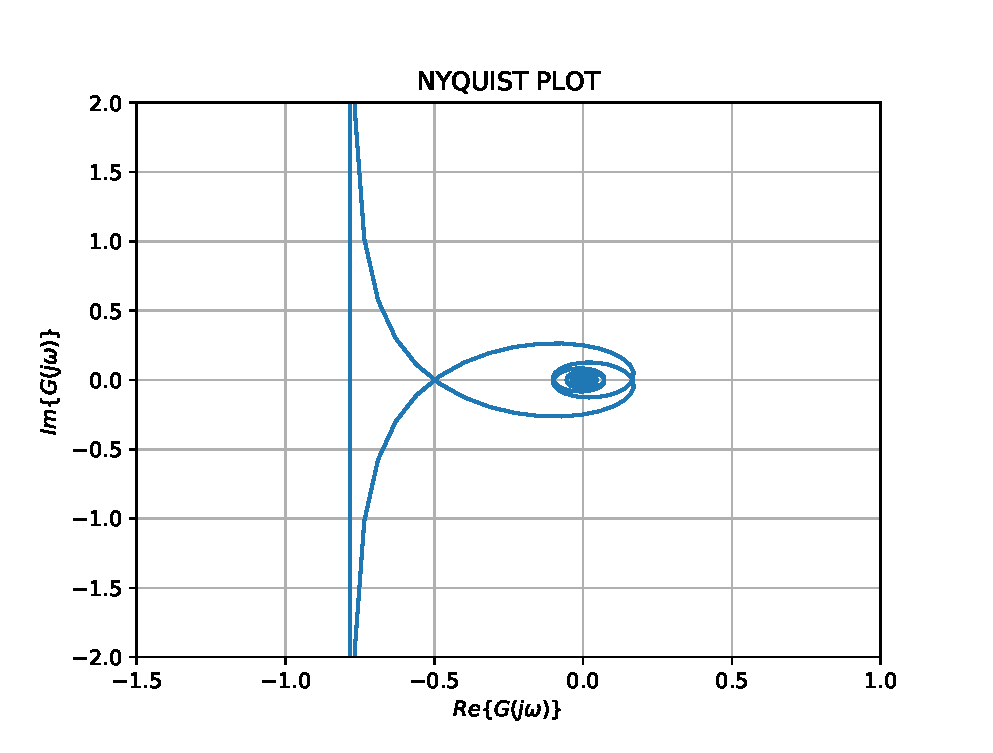
\includegraphics[width=\columnwidth]{ee18btech11007.eps}
  \caption{}
  \label{fig:ee18btech11007}
\end{figure}
%
\item Find the point at which the Nyquist plot of G(s) passes through the negative real axis
\\
\solution  Nyquist plot cuts the negative real axis at $\omega $ for which 
\begin{align}
\angle G(\j\omega)=-\pi
\label{eq:ee18btech11007_system_neg_real}
\end{align}
From \eqref{eq:ee18btech11007_system},
\begin{align}
 G(\j\omega)&=\frac{\pi e^{-\frac{\j\omega}{4}}}{\j\omega} = \frac{\pi e^{-\j\brak{\frac{\omega}{4}+\frac{\pi}{2}}}}{\omega}
\\
\implies \angle{ G(\j\omega)} &= -\brak{\frac{\omega}{4}+\frac{\pi}{2}}
\label{eq:ee18btech11007_system_ang}
\end{align}
From \eqref{eq:ee18btech11007_system_ang} and \eqref{eq:ee18btech11007_system_neg_real}, 
\begin{align}
\frac{\omega}{4}+\frac{\pi}{2} &= \pi
\\
\implies \omega = 2\pi
\end{align}
Also, from \eqref{eq:ee18btech11007_system},
\begin{align}
\label{eq:ee18btech11007_system_mod}
\abs{ G(\j\omega)}&=\frac{\pi }{\abs{\omega}}
\\
\implies \abs{ G(\j2\pi)} &= \frac{1}{2}
\end{align}
%
%\item Find the value of $P$ defined in Table \ref{table:ee18btech11007} from Fig.  \ref{fig:ee18btech11007}.

%
%\solution $P = 0$.
%\item Find the value of $N$ defined in Table \ref{table:ee18btech11007} from  \eqref{eq:ee18btech11007_system}
%\\
%\solution $\because H(s) = 1$, $G(s)H(s) = G(s)$. Also, $G(s)$ has a pole at $s = 0$, hence $N = 0$.
\item Use the Nyquist Stability criterion to determine if the system in \eqref{eq:ee18btech11007_system_ang} is stable.
\begin{table}[!ht]
\centering
%%%%%%%%%%%%%%%%%%%%%%%%%%%%%%%%%%%%%%%%%%%%%%%%%%%%%%%%%%%%%%%%%%%%%%
%%                                                                  %%
%%  This is the header of a LaTeX2e file exported from Gnumeric.    %%
%%                                                                  %%
%%  This file can be compiled as it stands or included in another   %%
%%  LaTeX document. The table is based on the longtable package so  %%
%%  the longtable options (headers, footers...) can be set in the   %%
%%  preamble section below (see PRAMBLE).                           %%
%%                                                                  %%
%%  To include the file in another, the following two lines must be %%
%%  in the including file:                                          %%
%%        \def\inputGnumericTable{}                                 %%
%%  at the beginning of the file and:                               %%
%%        \input{name-of-this-file.tex}                             %%
%%  where the table is to be placed. Note also that the including   %%
%%  file must use the following packages for the table to be        %%
%%  rendered correctly:                                             %%
%%    \usepackage[latin1]{inputenc}                                 %%
%%    \usepackage{color}                                            %%
%%    \usepackage{array}                                            %%
%%    \usepackage{longtable}                                        %%
%%    \usepackage{calc}                                             %%
%%    \usepackage{multirow}                                         %%
%%    \usepackage{hhline}                                           %%
%%    \usepackage{ifthen}                                           %%
%%  optionally (for landscape tables embedded in another document): %%
%%    \usepackage{lscape}                                           %%
%%                                                                  %%
%%%%%%%%%%%%%%%%%%%%%%%%%%%%%%%%%%%%%%%%%%%%%%%%%%%%%%%%%%%%%%%%%%%%%%



%%  This section checks if we are begin input into another file or  %%
%%  the file will be compiled alone. First use a macro taken from   %%
%%  the TeXbook ex 7.7 (suggestion of Han-Wen Nienhuys).            %%
\def\ifundefined#1{\expandafter\ifx\csname#1\endcsname\relax}


%%  Check for the \def token for inputed files. If it is not        %%
%%  defined, the file will be processed as a standalone and the     %%
%%  preamble will be used.                                          %%
\ifundefined{inputGnumericTable}

%%  We must be able to close or not the document at the end.        %%
	\def\gnumericTableEnd{\end{document}}


%%%%%%%%%%%%%%%%%%%%%%%%%%%%%%%%%%%%%%%%%%%%%%%%%%%%%%%%%%%%%%%%%%%%%%
%%                                                                  %%
%%  This is the PREAMBLE. Change these values to get the right      %%
%%  paper size and other niceties.                                  %%
%%                                                                  %%
%%%%%%%%%%%%%%%%%%%%%%%%%%%%%%%%%%%%%%%%%%%%%%%%%%%%%%%%%%%%%%%%%%%%%%

	\documentclass[12pt%
			  %,landscape%
                    ]{report}
       \usepackage[latin1]{inputenc}
       \usepackage{fullpage}
       \usepackage{color}
       \usepackage{array}
       \usepackage{longtable}
       \usepackage{calc}
       \usepackage{multirow}
       \usepackage{hhline}
       \usepackage{ifthen}

	\begin{document}


%%  End of the preamble for the standalone. The next section is for %%
%%  documents which are included into other LaTeX2e files.          %%
\else

%%  We are not a stand alone document. For a regular table, we will %%
%%  have no preamble and only define the closing to mean nothing.   %%
    \def\gnumericTableEnd{}

%%  If we want landscape mode in an embedded document, comment out  %%
%%  the line above and uncomment the two below. The table will      %%
%%  begin on a new page and run in landscape mode.                  %%
%       \def\gnumericTableEnd{\end{landscape}}
%       \begin{landscape}


%%  End of the else clause for this file being \input.              %%
\fi

%%%%%%%%%%%%%%%%%%%%%%%%%%%%%%%%%%%%%%%%%%%%%%%%%%%%%%%%%%%%%%%%%%%%%%
%%                                                                  %%
%%  The rest is the gnumeric table, except for the closing          %%
%%  statement. Changes below will alter the table's appearance.     %%
%%                                                                  %%
%%%%%%%%%%%%%%%%%%%%%%%%%%%%%%%%%%%%%%%%%%%%%%%%%%%%%%%%%%%%%%%%%%%%%%

\providecommand{\gnumericmathit}[1]{#1} 
%%  Uncomment the next line if you would like your numbers to be in %%
%%  italics if they are italizised in the gnumeric table.           %%
%\renewcommand{\gnumericmathit}[1]{\mathit{#1}}
\providecommand{\gnumericPB}[1]%
{\let\gnumericTemp=\\#1\let\\=\gnumericTemp\hspace{0pt}}
 \ifundefined{gnumericTableWidthDefined}
        \newlength{\gnumericTableWidth}
        \newlength{\gnumericTableWidthComplete}
        \newlength{\gnumericMultiRowLength}
        \global\def\gnumericTableWidthDefined{}
 \fi
%% The following setting protects this code from babel shorthands.  %%
 \ifthenelse{\isundefined{\languageshorthands}}{}{\languageshorthands{english}}
%%  The default table format retains the relative column widths of  %%
%%  gnumeric. They can easily be changed to c, r or l. In that case %%
%%  you may want to comment out the next line and uncomment the one %%
%%  thereafter                                                      %%
\providecommand\gnumbox{\makebox[0pt]}
%%\providecommand\gnumbox[1][]{\makebox}

%% to adjust positions in multirow situations                       %%
\setlength{\bigstrutjot}{\jot}
\setlength{\extrarowheight}{\doublerulesep}

%%  The \setlongtables command keeps column widths the same across  %%
%%  pages. Simply comment out next line for varying column widths.  %%
\setlongtables

\setlength\gnumericTableWidth{%
	55pt+%
	35pt+%
	119pt+%
0pt}
\def\gumericNumCols{3}
\setlength\gnumericTableWidthComplete{\gnumericTableWidth+%
         \tabcolsep*\gumericNumCols*2+\arrayrulewidth*\gumericNumCols}
\ifthenelse{\lengthtest{\gnumericTableWidthComplete > \linewidth}}%
         {\def\gnumericScale{\ratio{\linewidth-%
                        \tabcolsep*\gumericNumCols*2-%
                        \arrayrulewidth*\gumericNumCols}%
{\gnumericTableWidth}}}%
{\def\gnumericScale{1}}

%%%%%%%%%%%%%%%%%%%%%%%%%%%%%%%%%%%%%%%%%%%%%%%%%%%%%%%%%%%%%%%%%%%%%%
%%                                                                  %%
%% The following are the widths of the various columns. We are      %%
%% defining them here because then they are easier to change.       %%
%% Depending on the cell formats we may use them more than once.    %%
%%                                                                  %%
%%%%%%%%%%%%%%%%%%%%%%%%%%%%%%%%%%%%%%%%%%%%%%%%%%%%%%%%%%%%%%%%%%%%%%

\ifthenelse{\isundefined{\gnumericColA}}{\newlength{\gnumericColA}}{}\settowidth{\gnumericColA}{\begin{tabular}{@{}p{55pt*\gnumericScale}@{}}x\end{tabular}}
\ifthenelse{\isundefined{\gnumericColB}}{\newlength{\gnumericColB}}{}\settowidth{\gnumericColB}{\begin{tabular}{@{}p{35pt*\gnumericScale}@{}}x\end{tabular}}
\ifthenelse{\isundefined{\gnumericColC}}{\newlength{\gnumericColC}}{}\settowidth{\gnumericColC}{\begin{tabular}{@{}p{119pt*\gnumericScale}@{}}x\end{tabular}}

\begin{tabular}[c]{%
	b{\gnumericColA}%
	b{\gnumericColB}%
	b{\gnumericColC}%
	}

%%%%%%%%%%%%%%%%%%%%%%%%%%%%%%%%%%%%%%%%%%%%%%%%%%%%%%%%%%%%%%%%%%%%%%
%%  The longtable options. (Caption, headers... see Goosens, p.124) %%
%	\caption{The Table Caption.}             \\	%
% \hline	% Across the top of the table.
%%  The rest of these options are table rows which are placed on    %%
%%  the first, last or every page. Use \multicolumn if you want.    %%

%%  Header for the first page.                                      %%
%	\multicolumn{3}{c}{The First Header} \\ \hline 
%	\multicolumn{1}{c}{colTag}	%Column 1
%	&\multicolumn{1}{c}{colTag}	%Column 2
%	&\multicolumn{1}{c}{colTag}	\\ \hline %Last column
%	\endfirsthead

%%  The running header definition.                                  %%
%	\hline
%	\multicolumn{3}{l}{\ldots\small\slshape continued} \\ \hline
%	\multicolumn{1}{c}{colTag}	%Column 1
%	&\multicolumn{1}{c}{colTag}	%Column 2
%	&\multicolumn{1}{c}{colTag}	\\ \hline %Last column
%	\endhead

%%  The running footer definition.                                  %%
%	\hline
%	\multicolumn{3}{r}{\small\slshape continued\ldots} \\
%	\endfoot

%%  The ending footer definition.                                   %%
%	\multicolumn{3}{c}{That's all folks} \\ \hline 
%	\endlastfoot
%%%%%%%%%%%%%%%%%%%%%%%%%%%%%%%%%%%%%%%%%%%%%%%%%%%%%%%%%%%%%%%%%%%%%%

\hhline{|-|-|-}
	 \multicolumn{1}{|p{\gnumericColA}|}%
	{\gnumericPB{\centering}\textbf{Variable}}
	&\multicolumn{1}{p{\gnumericColB}|}%
	{\gnumericPB{\centering}\textbf{Value}}
	&\multicolumn{1}{p{\gnumericColC}|}%
	{\gnumericPB{\raggedright}\textbf{Description}}
\\
\hhline{|---|}
	 \multicolumn{1}{|p{\gnumericColA}|}%
	{\gnumericPB{\centering}Z}
	&\multicolumn{1}{p{\gnumericColB}|}%
	{\gnumericPB{\centering}0}
	&\multicolumn{1}{p{\gnumericColC}|}%
	{\gnumericPB{\raggedright}Poles of $\frac{G(s)}{1+G(s)H(s)}$in right half of s plane}
\\
\hhline{|---|}
	 \multicolumn{1}{|p{\gnumericColA}|}%
	{\gnumericPB{\centering}P}
	&\multicolumn{1}{p{\gnumericColB}|}%
	{\gnumericPB{\centering}0}
	&\multicolumn{1}{p{\gnumericColC}|}%
	{\gnumericPB{\raggedright}Poles of $G(s)H(s)$ in right half of s plane}
\\
\hhline{|---|}
	 \multicolumn{1}{|p{\gnumericColA}|}%
	{\gnumericPB{\centering}N}
	&\multicolumn{1}{p{\gnumericColB}|}%
	{\gnumericPB{\centering}0}
	&\multicolumn{1}{p{\gnumericColC}|}%
	{\gnumericPB{\raggedright}No of clockwise encirclements of $G(s)H(s)$  about -1+j0 in the Nyquist plot}
\\
\hhline{|-|-|-|}
\end{tabular}

\ifthenelse{\isundefined{\languageshorthands}}{}{\languageshorthands{\languagename}}
\gnumericTableEnd


\caption{}
\label{table:EE18btech11007}
\end{table}
\\
\solution Consider Table \ref{table:EE18btech11007}.  According to the Nyquist stability criterion, 
\begin{enumerate}
\item If the open-loop transfer function $G(s)$ has a zero pole of multiplicity $l$, then the Nyquist plot has a discontinuity at $\omega$ =0. During further analysis it should be assumed that the phasor travels l times clock-wise along a semicircle of infinite radius. After applying this rule, the zero poles should be neglected, i.e. if there are no other unstable poles, then the open-loop transfer function $G(s)$ should be considered stable.
\item If the open-loop transfer function $G(s)$ is stable, then the closed-loop system is unstable for any encirclement of the point -1.
If the open-loop transfer function $G(s)$ is unstable, then there must be one counter clock-wise encirclement of -1 for each pole of $G(s)$ in the right-half of the complex plane.
\label{them:ee18btech11007_nyquist3}
\item The number of surplus encirclements (N + P greater than 0) is exactly the number of unstable poles of the closed-loop system.
\item However, if the graph happens to pass through the point $-1+\j0$, then deciding upon even the marginal stability of the system becomes difficult and the only conclusion that can be drawn from the graph is that there exist zeros on the $\j \omega$  axis.
\end{enumerate}
From \eqref{eq:ee18btech11007_system}, $G(s)$ is stable since it has a single pole at $s = 0$.  Further,  from Fig.  \ref{fig:ee18btech11007}, the Nyquist plot does not encircle $s =  -1$.  From  Theorem \ref{them:ee18btech11007_nyquist3}, we may conclude that the system is stable.


\end{enumerate}

